\usepackage{amsthm}

\newtheorem{theorem}{Theorem}[chapter]
\newtheorem{lemma}           [theorem] {Lemma}   
\newtheorem{folg}           [theorem] {Folgerung}   

\newtheorem{frage}       [theorem] {Frage}   
\newtheorem{question}       [theorem] {Question}   
\newtheorem{aufgabe}       [theorem] {Aufgabe}   
\newtheorem{exercise}       [theorem] {Exercise}  

\newtheorem{proposition}     [theorem] {Proposition}  
\newtheorem{satz}     [theorem] {Satz}  
\newtheorem{fact}{Fact}
\newtheorem{definition}      [theorem] {Definition} 

\theoremstyle{definition} 
\newtheorem{bemerkung}     [theorem] {Bemerkung}  
\newtheorem{beispiel}       [theorem] {Beispiel}  
\newtheorem{example}       [theorem] {Example}  
\newtheorem*{example*} {Example}  
\newtheorem{notation}       [theorem] {Notation}  
\newtheorem*{Faust}[theorem]{Rule of Thumb}
\newtheorem*{Boxx}[theorem]{Concept}

\begin{Theorem}[$\varepsilon$-$\delta$ criterion for continuity]
Let $I\subset \mathbb{K}$ and $f:I\to\mathbb{K}$ be a~function. Let $x_0\in I$. Then the following two statements are equivalent.
\begin{enumerate}[(i)]
 \item $f$ is continuous in $x_0$;
 \item For all $\varepsilon>0$ there exists some $\delta>0$ such that for all $x\in I$ with $|x-x_0|<\delta$ holds
\[|f(x)-f(x_0)|<\varepsilon.\]
\end{enumerate}
\end{Theorem}

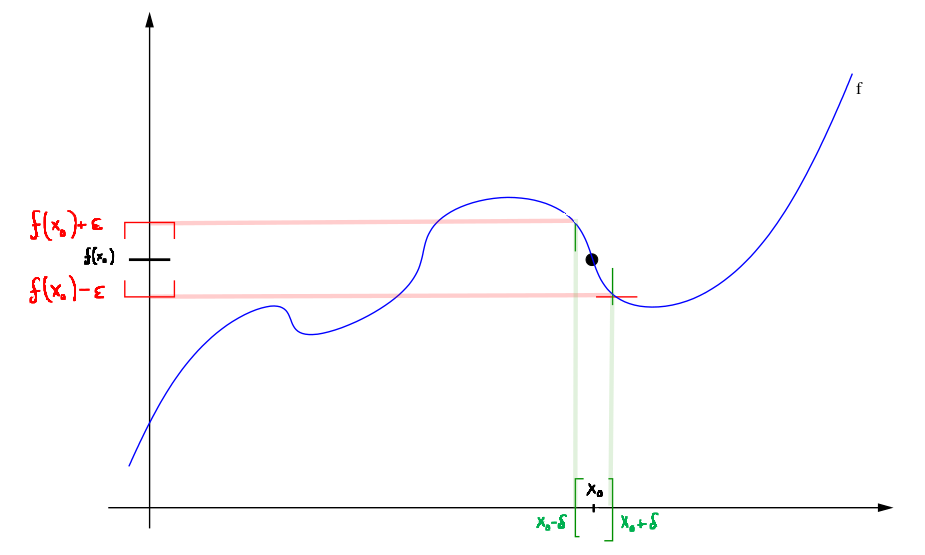
\includegraphics{./eps.png}

{\em Proof:}\\
``(i)$\Rightarrow$(ii)'': Assume that (ii) is not fulfilled, i.e., there exists some $\varepsilon>0$, such that for all $\delta>0$, there exists some $x\in I\setminus\{x_{0}\}$ with $|x-x_0|<\delta$ and $|f(x)-f(x_0)|>\varepsilon$. As a~consequence, for all $n\in\mathbb{N}$, there exists some $x_n\in I\setminus\{x_{0}\}$ with
\[|x_0-x_n|<\frac1n\;\text{ and }\;|f(x_n)-f(x_0)|>\varepsilon.\]
Therefore, the sequence $(x_n)_{n\in\mathbb{N}}$ converges to $x_0$, but $|f(x_n)-f(x_0)|>\varepsilon$,
i.e., $f(x_n)$ is not converging to $f(x_0)$.\\
``(ii)$\Rightarrow$(i)'': Let  $(x_n)_{n\in\mathbb{N}}$ be a~sequence in $I\backslash\{x_0\}$ that converges to $x_0$. Let $\varepsilon>0$. Then there exists some $\delta>0$ such that for all $x\in I$ with $|x-x_0|<\delta$ holds $|f(x)-f(x_0)|<\varepsilon$. Since $(x_n)_{n\in\mathbb{N}}$ converges to $x_0$, there exists some $N$ such that for all $n\geq N$ holds $|x_n-x_0|<\delta$. By the $\varepsilon$-$\delta$-criterion, we have then for all $n\geq N$ that
\[|f(x_n)-f(x_0)|<\varepsilon.\]
Hence, $(f(x_n))_{n\in\mathbb{N}}$ converges to $f(x_0)$.\hfill$\Box$

